\section*{Annexes}
\addcontentsline{toc}{chapter}{Annexes}

%\section{Détails des objectifs et actions liées à l'écoresponsabilité}
\begin{table}[ht]
    \centering
    \begin{tabular}{|p{4,5cm}|p{10,5cm}|}
    \hline
    \textbf{Les principaux postes d’émissions identifiés} & \textbf{Quelques objectifs et actions} \\
    \hline
    Missions & 
    - Prévention sur le sujet sur le site Carbon Footprint du Cerfacs et affiches présentes dans les locaux. \\
    \hline
    Chauffage & 
    - Rénovation du circuit d’alimentation en eau glacée des ventilo-convecteurs de l’ancien bâtiment (Actions 2023 et 2024) \newline
    - Traitement de l’étanchéité et de l’isolation de l’ancien bâtiment (analyse réalisée, actions en cours réparties sur plusieurs années pour cause de coût global). \\
    \hline
    Calculateurs internes et usage & 
    - Un calculateur a été arrêté en février 2023 et remplacé seulement en 2024. \newline
    - Une sensibilisation à l’optimisation de l’usage des calculateurs \\
    \hline
    Calculateurs internes et \\fabrication &  \\
    \hline
    Électricité hors clusters & 
    - Automatisation de l’éclairage des circulations de l’ancien bâtiment (abandon de l’éclairage manuel). \\
    \hline
    Trajet domicile-travail & 
    - Participation à des initiatives en faveur du vélo ("Deux Pieds Deux Roues - 2P2R", "Objectif Employeur Pro Vélo") \newline
    - Mise en place du Forfait Mobilité Durable pour le vélo. \newline
    - Mise à disposition de deux vélos pour le personnel du Cerfacs \\
    \hline
    Fuites de fluides &  \\
    \hline
    Calculateurs externes et usage & 
    - Une sensibilisation à l’optimisation de l’usage des calculateurs \\
    \hline
    Calculateurs externes et \\fabrication &  \\
    \hline
    Matériel informatique & 
    Les postes de travail sont globalement à jour et ont un bon niveau de technologie (77\% publiés en 2023). \\
    \hline
    \end{tabular}
    \caption{Axes de travail et exemples d'actions pour limiter l'empreinte carbone du CERFACS}
    \label{tab:Eco_actions}
\end{table}


%\section{Détails des actions liées à la Qualité de Vie au Travail}

\begin{table}[ht]
    \centering
    \begin{tabular}{|p{5cm}|p{10cm}|}
    \hline
    \textbf{Axes de travail} & \textbf{Exemples d’actions} \\
    \hline
    Optimiser l’organisation et gestion du travail au niveau global & 
    - Organisation d’une réunion générale du Cerfacs par la direction 2 fois par an \newline
    - Valorisation de la bibliothèque (réaménagement de l’espace) \newline
    - Amélioration de la communication interne (journal de la QVT disponible sur l’intranet, newsletter interne mensuelle) et externe (nomination d’un référent Communication) \\
    \hline
    Optimiser l’organisation et gestion du travail au niveau de l’équipe & 
    - Proposer une formation à l’organisation et à la tenue de réunions efficaces \\
    \hline
    Optimiser l’organisation et gestion du travail au niveau personnel & 
    - Information/sensibilisation au burn-out (par la médecine du travail) \\
    \hline
    Assurer un meilleur accueil et support des non permanents & 
    - Mise en place d’un groupe de travail pour optimiser l’encadrement des non-permanents (doctorants, post-doctorants…) \newline
    - Rédaction d’une charte QVT \\
    \hline
    Favoriser la vie sociale & 
    - Organisation d’événements sociaux en dehors du temps de travail \newline
    - Aménagement d’une salle de repos \newline
    - Organisation de pauses café collectives mensuelles \\
    \hline
    Améliorer le confort matériel & 
    - Nouvelle machine à café à grain mise à disposition pour tous (avec l’achat de café par le Cerfacs) \newline
    - Gourdes métalliques offertes à l’ensemble du personnel \newline
    - Achat et installation de nouveaux arceaux pour augmenter la capacité d’accueil des vélos \newline
    - Sensibilisation à l’ergonomie sur le poste de travail (par la médecine du travail) \\
    \hline
    \end{tabular}
    \caption{Axes de travail et exemples d'actions pour la Qualité de Vie au Travail au CERFACS}
    \label{tab:QVT_actions}
\end{table}


\begin{figure}[ht]
    \centering
    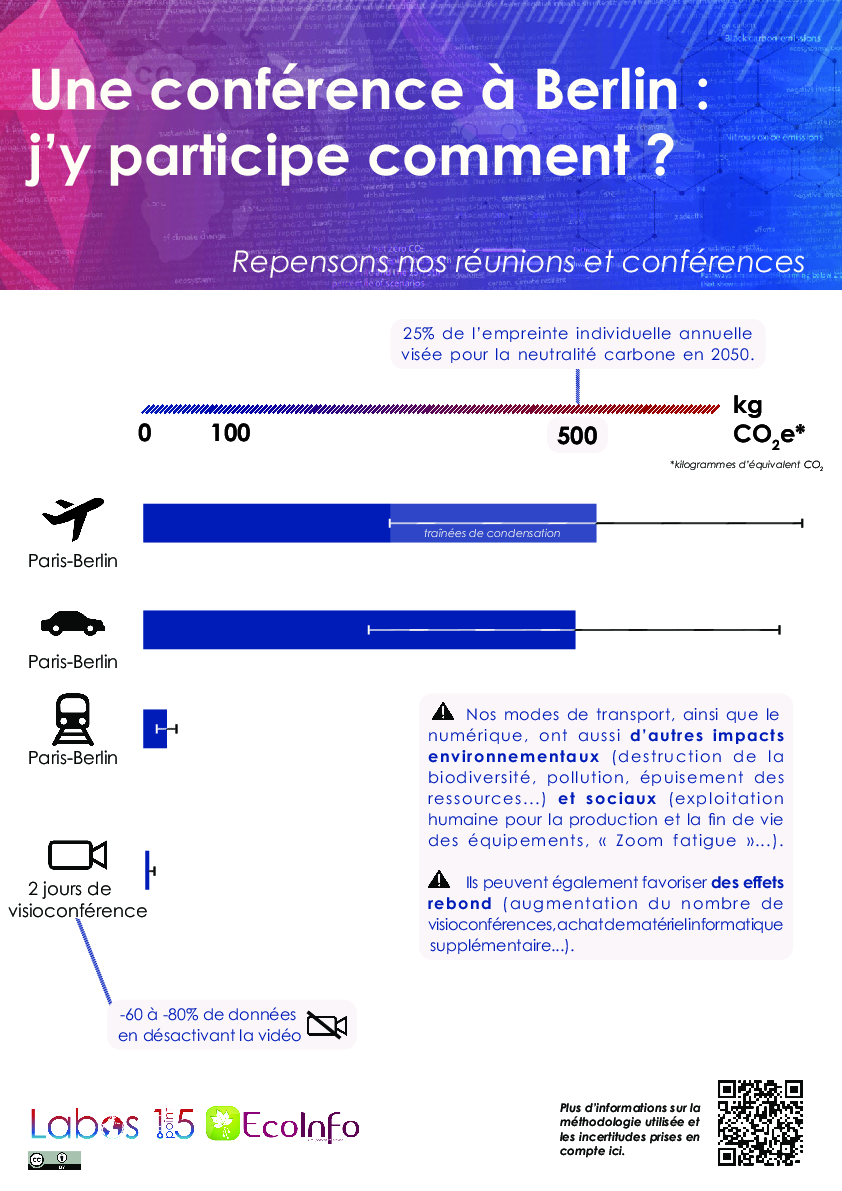
\includegraphics[width=0.5\textwidth]{images/berlin_v7_fr.png}
    \caption{Empreinte carbone s'une conférence à Berlin}
    \label{fig:berlin}
\end{figure}

\begin{figure}[ht]
    \centering
    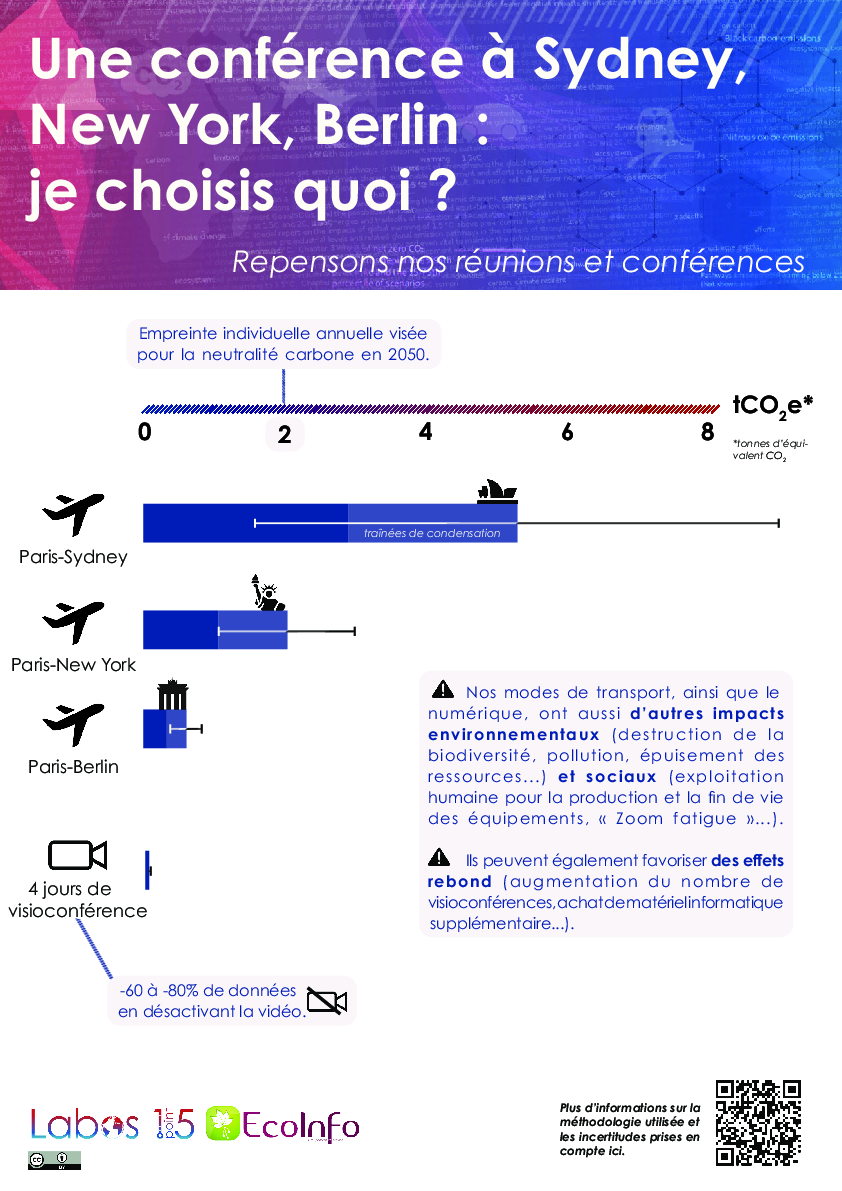
\includegraphics[width=0.5\textwidth]{images/sydney_v7_fr.png}
    \caption{Empreinte carbone s'une conférence à Sydney}
    \label{fig:sydney}
\end{figure}